% ANEXOS
% Este archivo contiene los diagramas y mockups del sistema

%----------------------------------------------------------------------------------------
% ANEXO A: DIAGRAMAS DE ARQUITECTURA Y DISEÑO
%----------------------------------------------------------------------------------------
\section{Diagramas de Arquitectura y Diseño del Sistema}
\label{anexo:diagramas}

Esta sección presenta los diagramas técnicos que ilustran la arquitectura, diseño y funcionamiento del sistema desarrollado.

\subsection{Diagrama de Contexto}
\label{anexo:diagrama_contexto}

El diagrama de contexto muestra la visión general del sistema y sus interacciones con actores externos.

\begin{figure}[h]
\centering
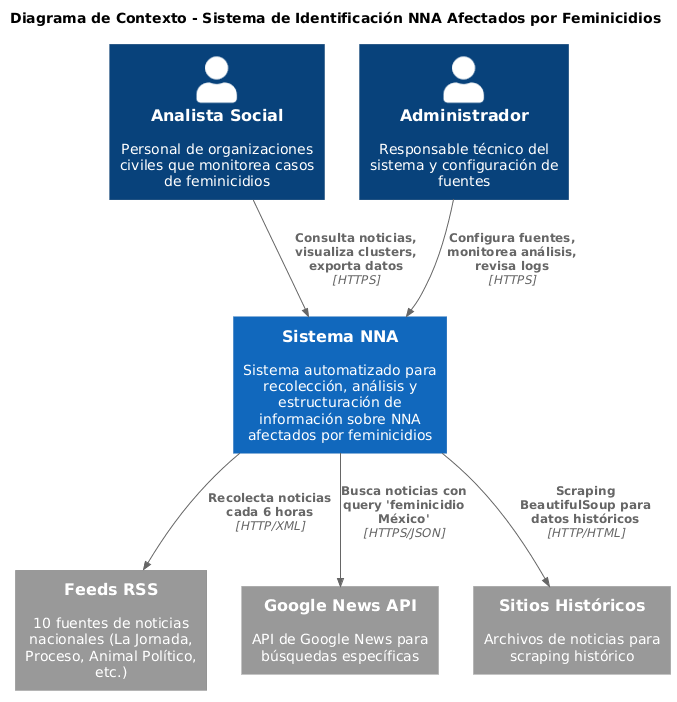
\includegraphics[width=0.75\textwidth,keepaspectratio]{media/Diagrama_contexto.png}
\caption{Diagrama de contexto del sistema}
\label{fig:diagrama_contexto}
\end{figure}

\subsection{Diagrama de Casos de Uso}
\label{anexo:diagrama_casos_uso}

Este diagrama representa los casos de uso principales del sistema y las interacciones de los usuarios con el mismo.

\begin{figure}[h]
\centering
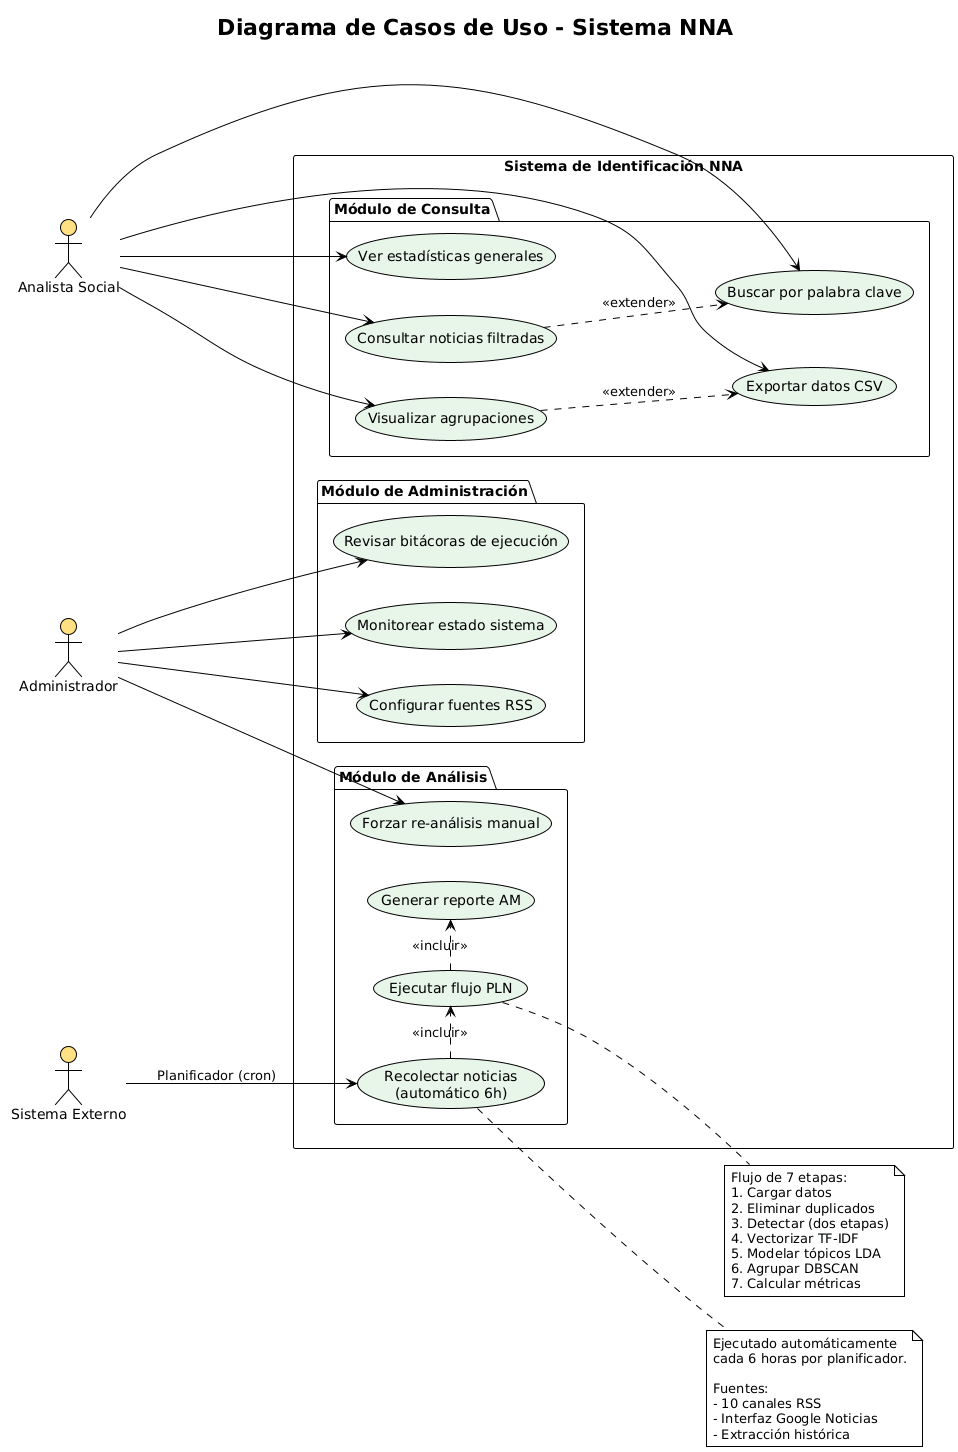
\includegraphics[width=0.75\textwidth,keepaspectratio]{media/Diagrama_casosUsos.png}
\caption{Diagrama de casos de uso del sistema}
\label{fig:diagrama_casos_uso}
\end{figure}

\subsection{Diagrama de Componentes}
\label{anexo:diagrama_componentes}

El diagrama de componentes muestra la estructura modular del sistema y las relaciones entre sus componentes principales.

\begin{figure}[h]
\centering
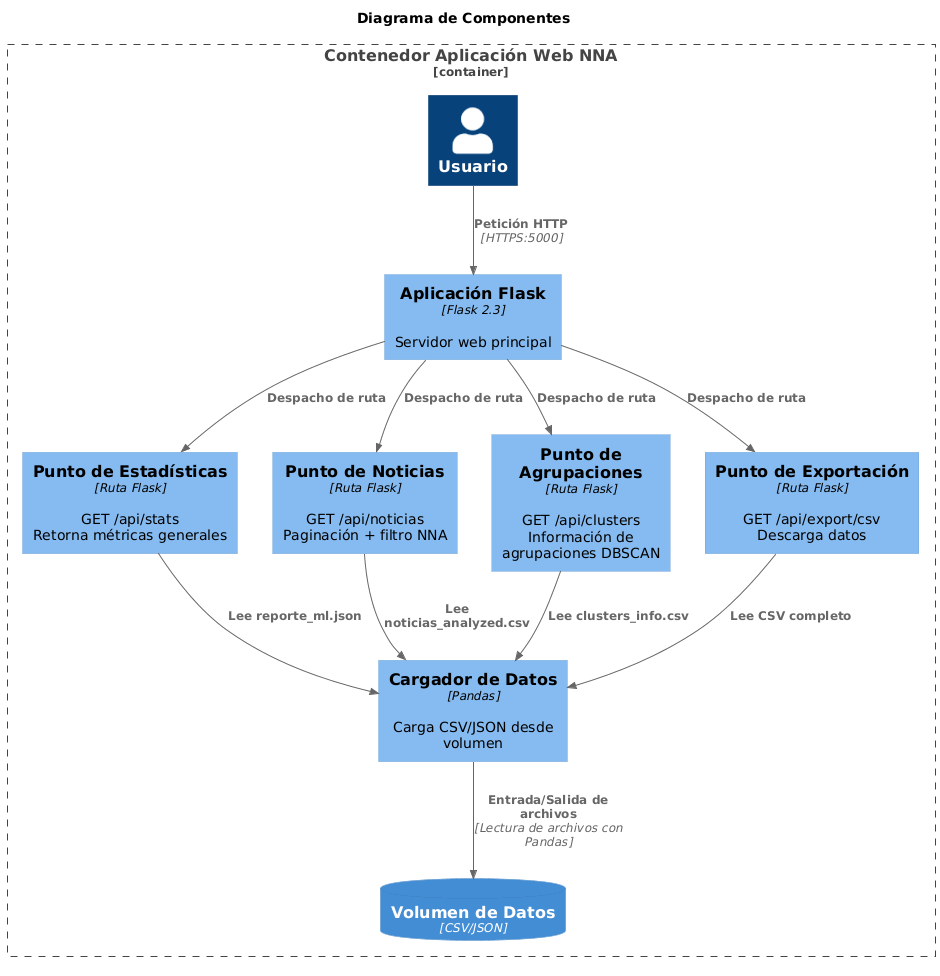
\includegraphics[width=0.75\textwidth,keepaspectratio]{media/Diagrama_componentes.png}
\caption{Diagrama de componentes del sistema}
\label{fig:diagrama_componentes}
\end{figure}

\subsection{Diagrama de Componentes de Análisis}
\label{anexo:diagrama_componentes_analisis}

Detalle de los componentes específicos del módulo de análisis de noticias.

\begin{figure}[p]
\centering
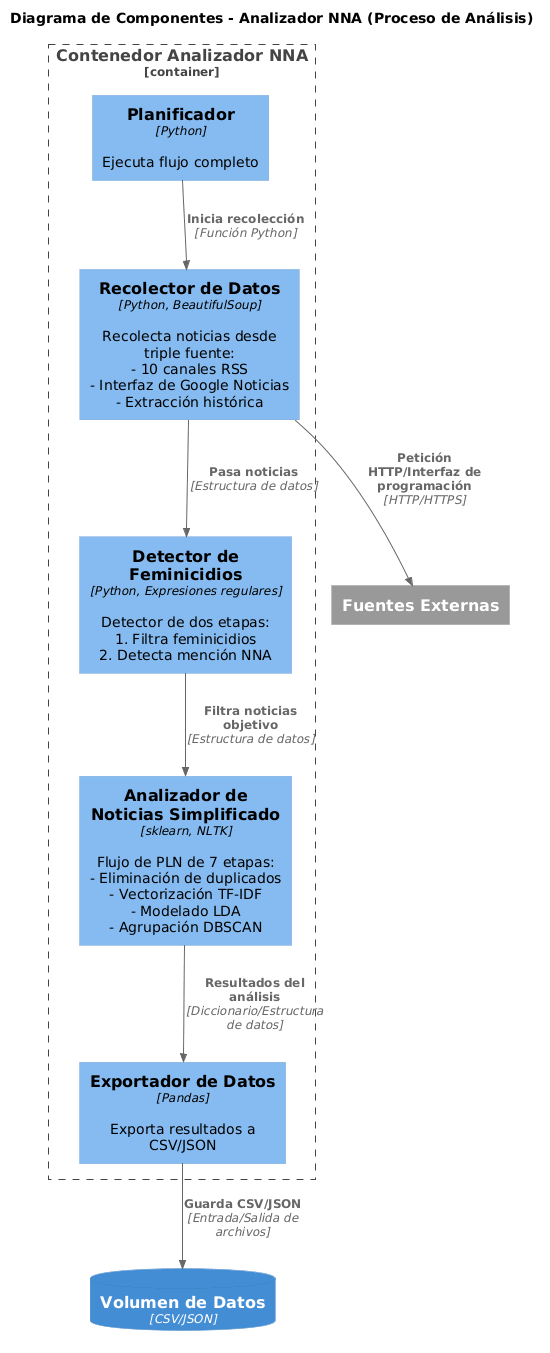
\includegraphics[height=0.85\textheight,keepaspectratio]{media/Diagrama_componentesAnalisis.png}
\caption{Diagrama de componentes del módulo de análisis}
\label{fig:diagrama_componentes_analisis}
\end{figure}

\clearpage

%----------------------------------------------------------------------------------------
% ANEXO B: DIAGRAMAS DE FLUJO Y PROCESOS
%----------------------------------------------------------------------------------------
\section{Diagramas de Flujo y Procesos}
\label{anexo:diagramas_flujo}

\subsection{Diagrama de Flujo Completo del Sistema}
\label{anexo:flujo_completo}

Este diagrama muestra el flujo completo de procesamiento de información en el sistema, desde la recolección hasta la presentación de resultados.

\begin{figure}[h]
\centering
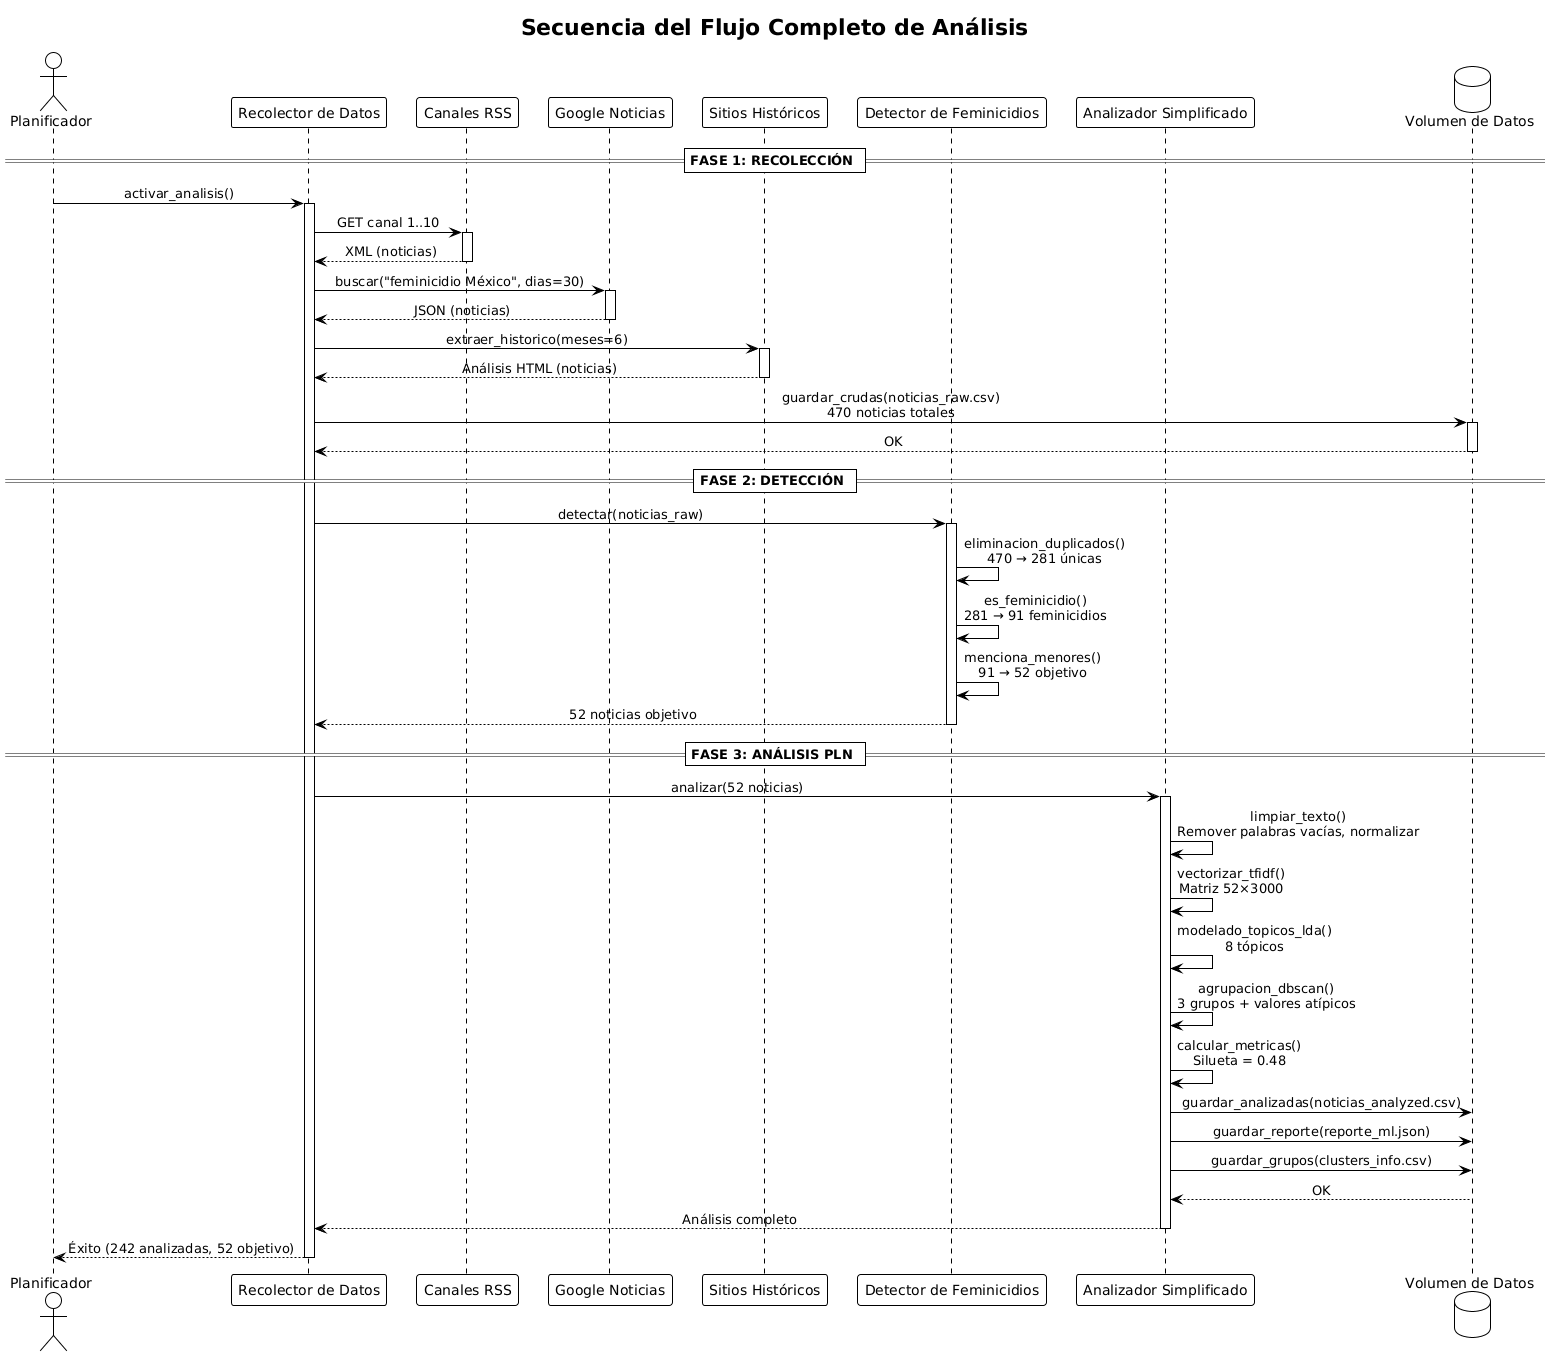
\includegraphics[width=0.7\textwidth,keepaspectratio]{media/Diagra_flujoCompleto.png}
\caption{Diagrama de flujo completo del sistema}
\label{fig:flujo_completo}
\end{figure}

\subsection{Diagrama de flujo de metodologías}
\label{anexo:flujo_pnl}

Detalle del flujo de las metodologías aplicadasa las noticias recolectadas.

\begin{figure}[p]
\centering
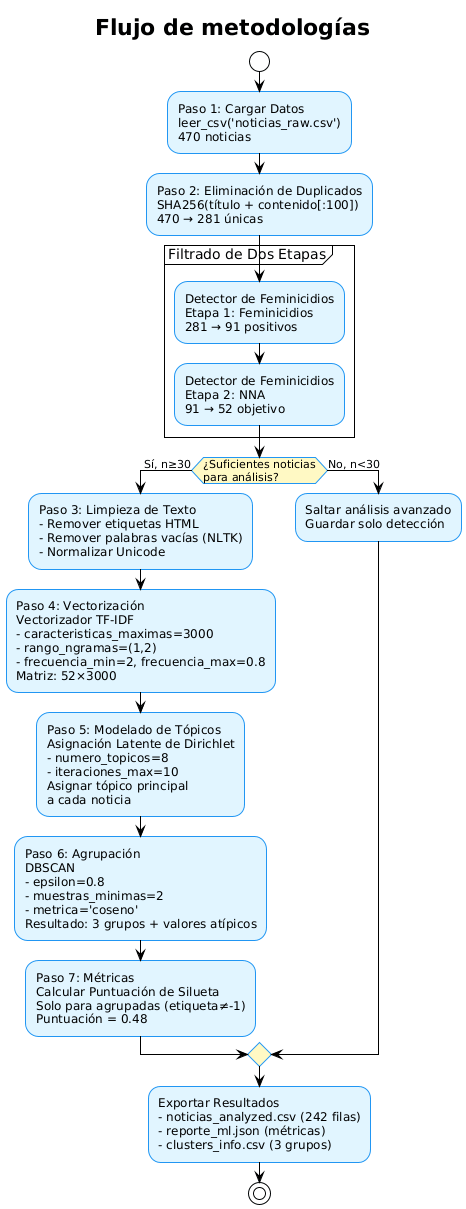
\includegraphics[height=0.85\textheight,keepaspectratio]{media/Diagrama_flujoPNL.png}
\caption{Diagrama de flujo de metodologías}
\label{fig:flujo_pnl}
\end{figure}

\subsection{Diagrama del Detector de Dos Etapas}
\label{anexo:detector_dos_etapas}

Diagrama que ilustra el funcionamiento del detector especializado de feminicidios con menciones de NNA, implementado en dos etapas para reducir falsos positivos.

\begin{figure}[h]
\centering
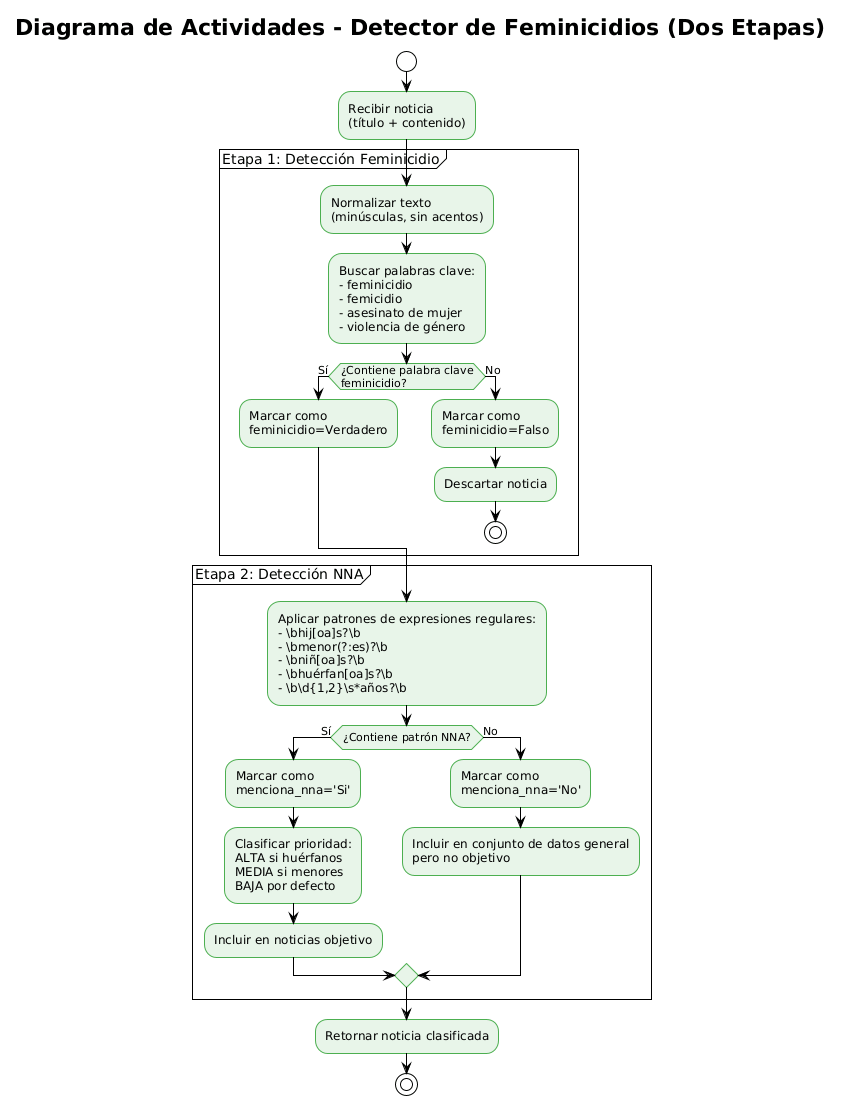
\includegraphics[width=0.7\textwidth,keepaspectratio]{media/Diagrama_detectorDosEtapas.png}
\caption{Diagrama del detector de feminicidios en dos etapas}
\label{fig:detector_dos_etapas}
\end{figure}

\clearpage

%----------------------------------------------------------------------------------------
% ANEXO C: ARQUITECTURA DOCKER Y EVOLUCIÓN
%----------------------------------------------------------------------------------------
\section{Arquitectura de Contenedores y Evolución del Sistema}
\label{anexo:docker_evolucion}

\subsection{Arquitectura Docker}
\label{anexo:arquitectura_docker}

Diagrama de la arquitectura de contenedores Docker implementada para el despliegue del sistema.

\begin{figure}[h]
\centering
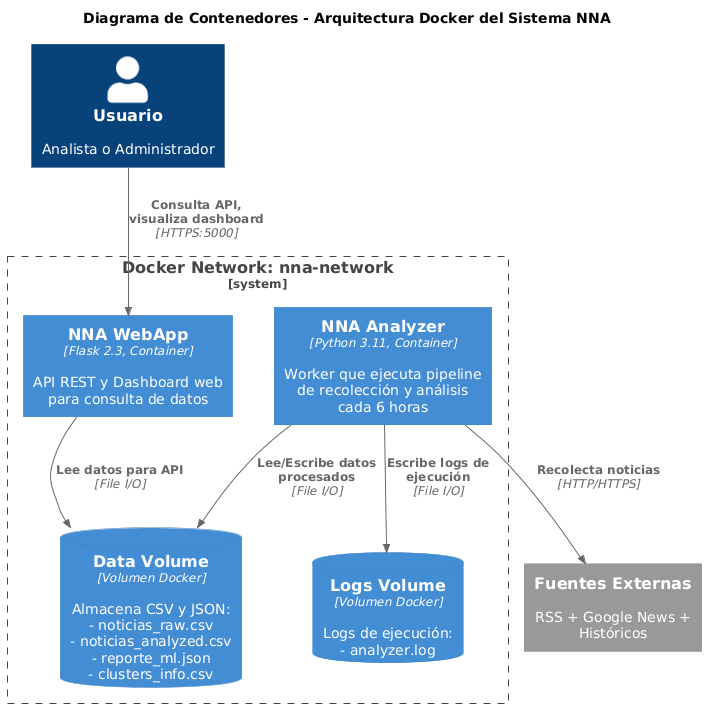
\includegraphics[width=0.75\textwidth,keepaspectratio]{media/Diagrama_docker.png}
\caption{Arquitectura Docker del sistema}
\label{fig:arquitectura_docker}
\end{figure}

\subsection{Evolución de Prototipos}
\label{anexo:evolucion_prototipos}

Diagrama que muestra la evolución del sistema a través de los diferentes prototipos desarrollados (P0, P1, P2).

\begin{figure}[h]
\centering
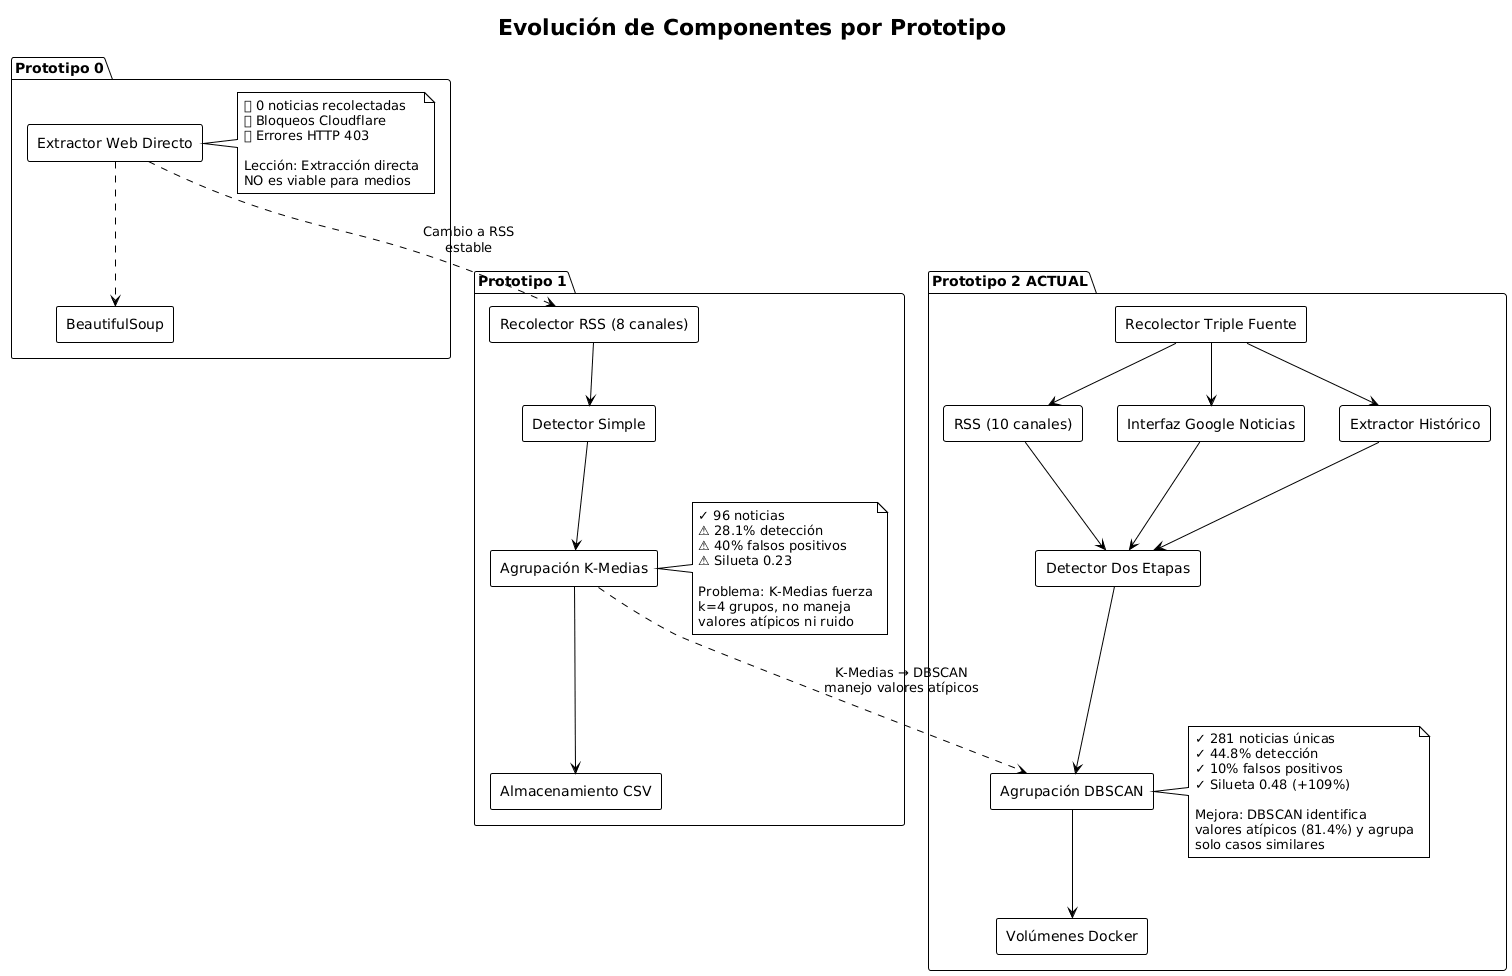
\includegraphics[width=0.75\textwidth,keepaspectratio]{media/Diagrama_evolucion.png}
\caption{Evolución de prototipos del sistema}
\label{fig:evolucion_prototipos}
\end{figure}

\clearpage

%----------------------------------------------------------------------------------------
% ANEXO D: MOCKUPS DE INTERFAZ DE USUARIO
%----------------------------------------------------------------------------------------
\section{Mockups de Interfaz de Usuario}
\label{anexo:mockups}

Esta sección presenta los diseños de interfaz de usuario del sistema.

\subsection{Mockup de Pantalla de Login}
\label{anexo:mockup_login}

Diseño de la pantalla de inicio de sesión del sistema.

\begin{figure}[h]
\centering
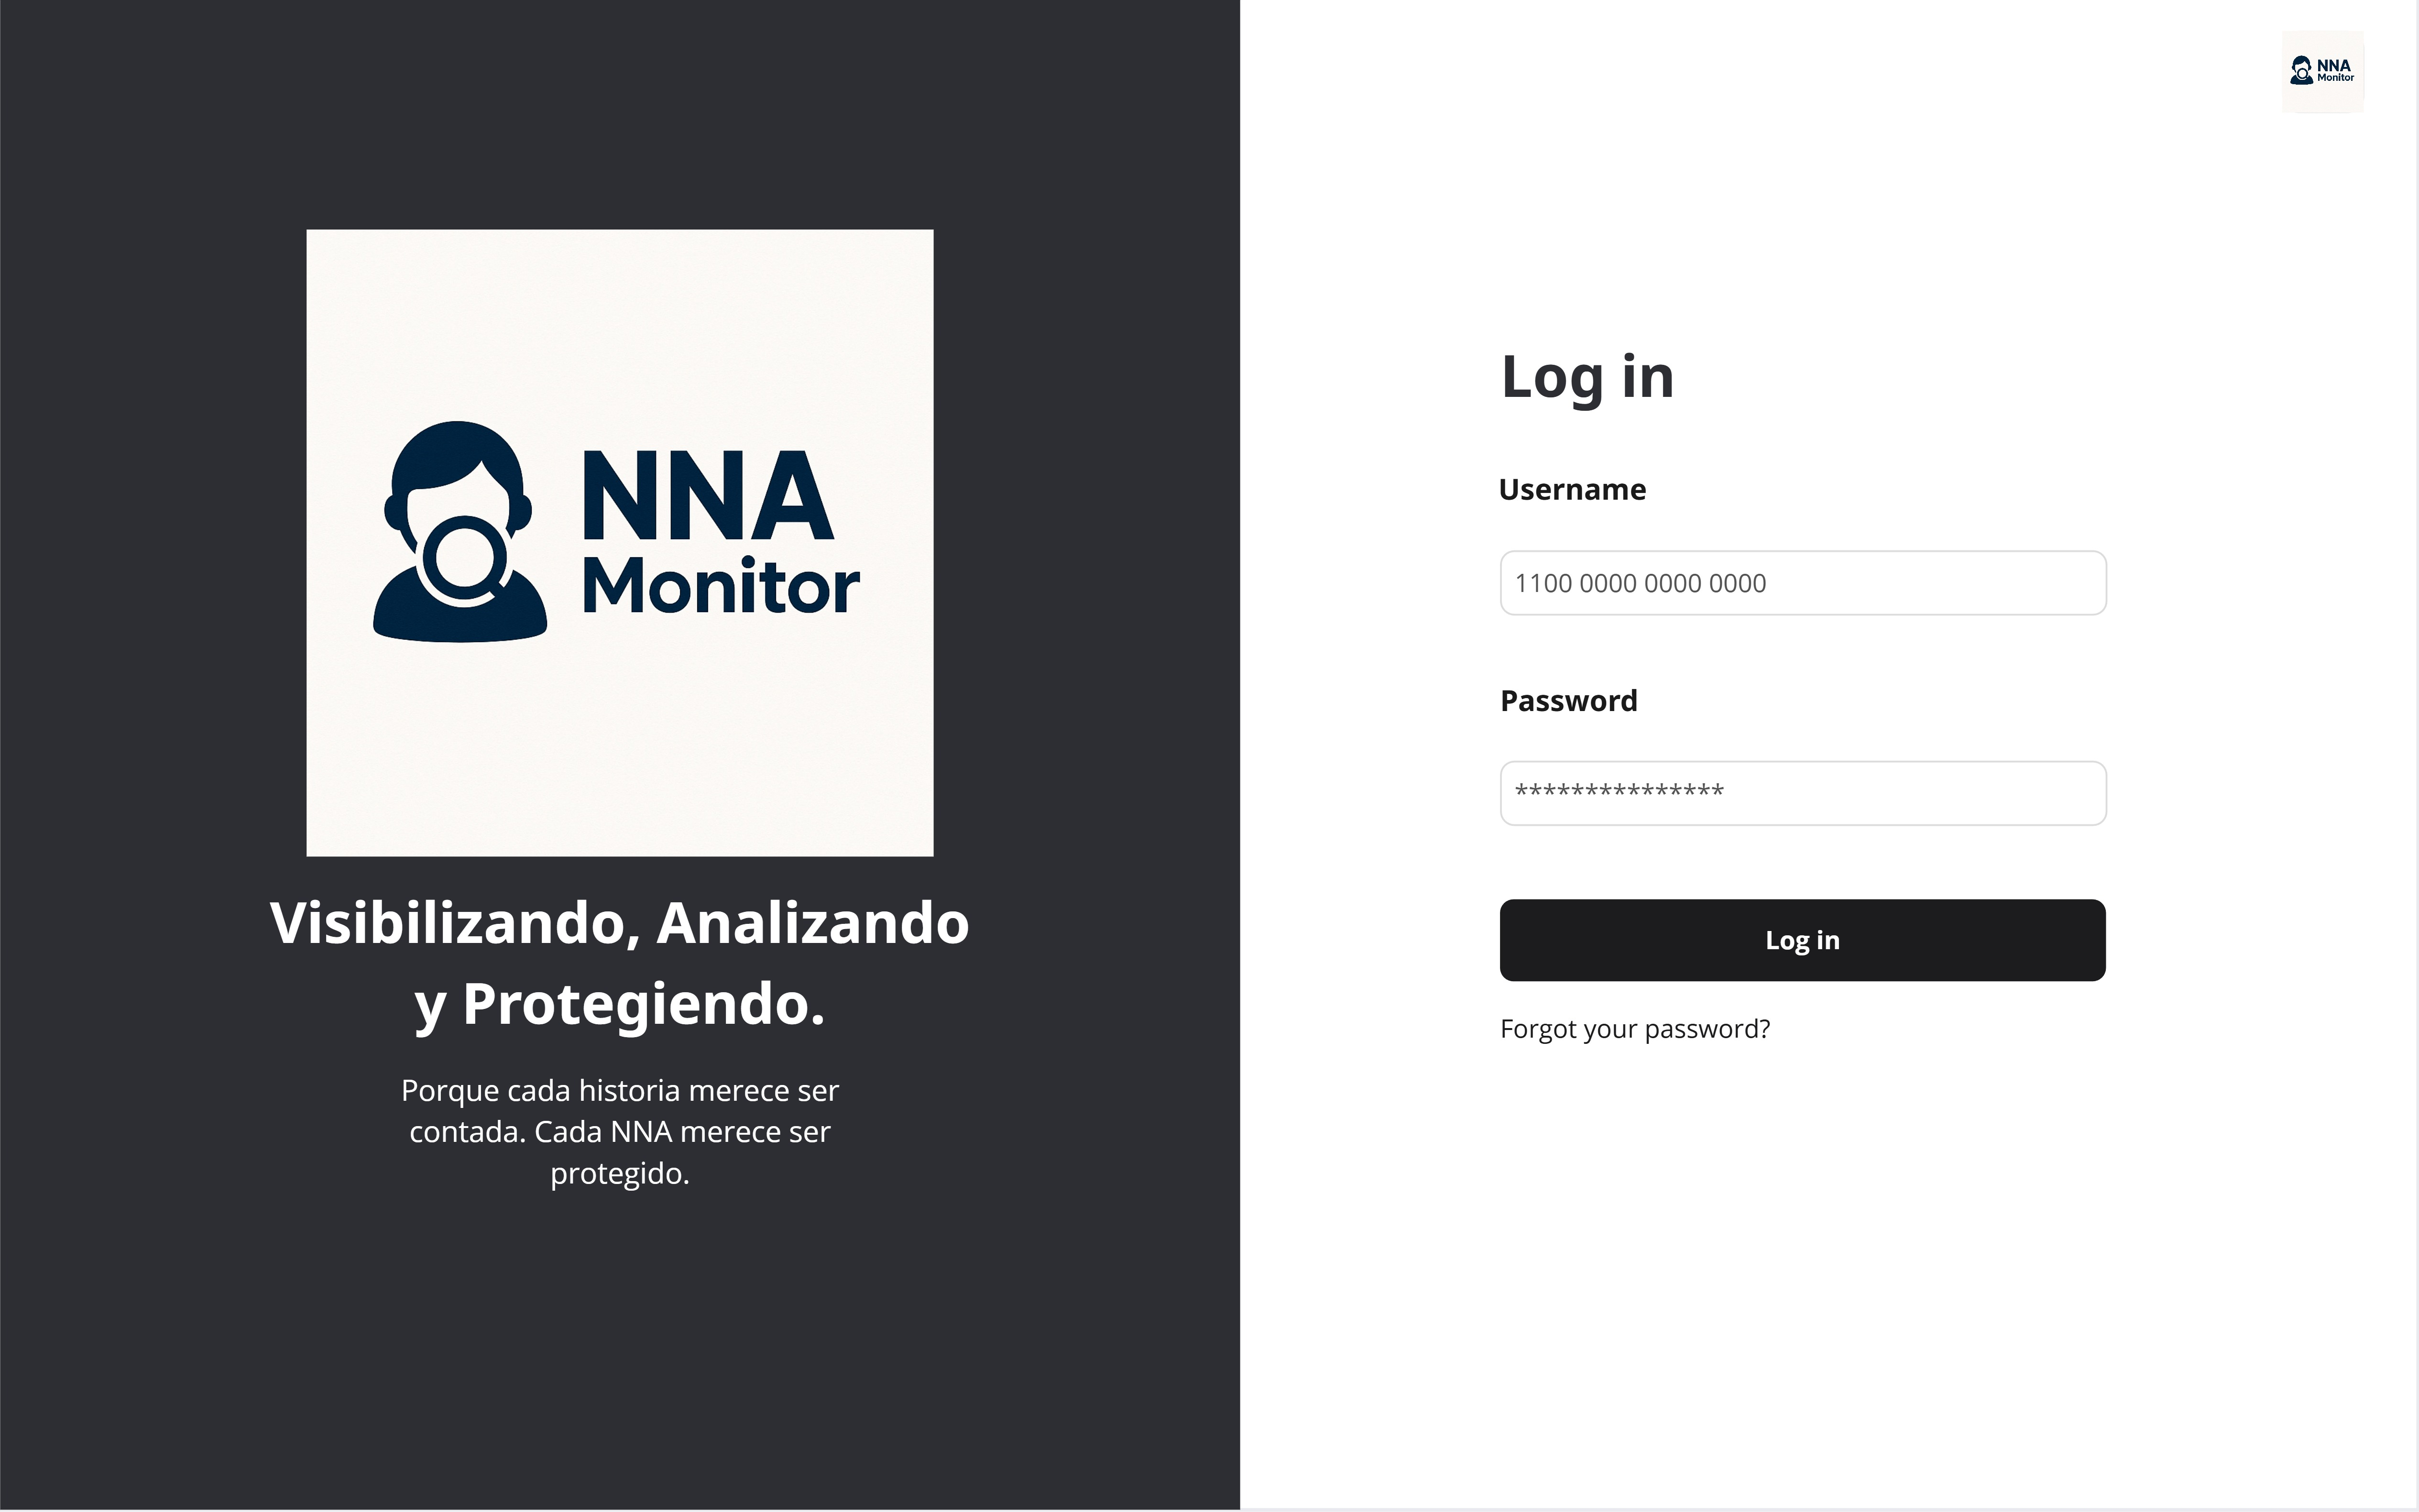
\includegraphics[width=0.7\textwidth,keepaspectratio]{media/Mockup_login.jpg}
\caption{Mockup de la pantalla de login}
\label{fig:mockup_login}
\end{figure}

\subsection{Mockup de Pantalla Principal (Home)}
\label{anexo:mockup_home}

Diseño de la pantalla principal del sistema donde se visualiza el dashboard con la información general.

\begin{figure}[h]
\centering
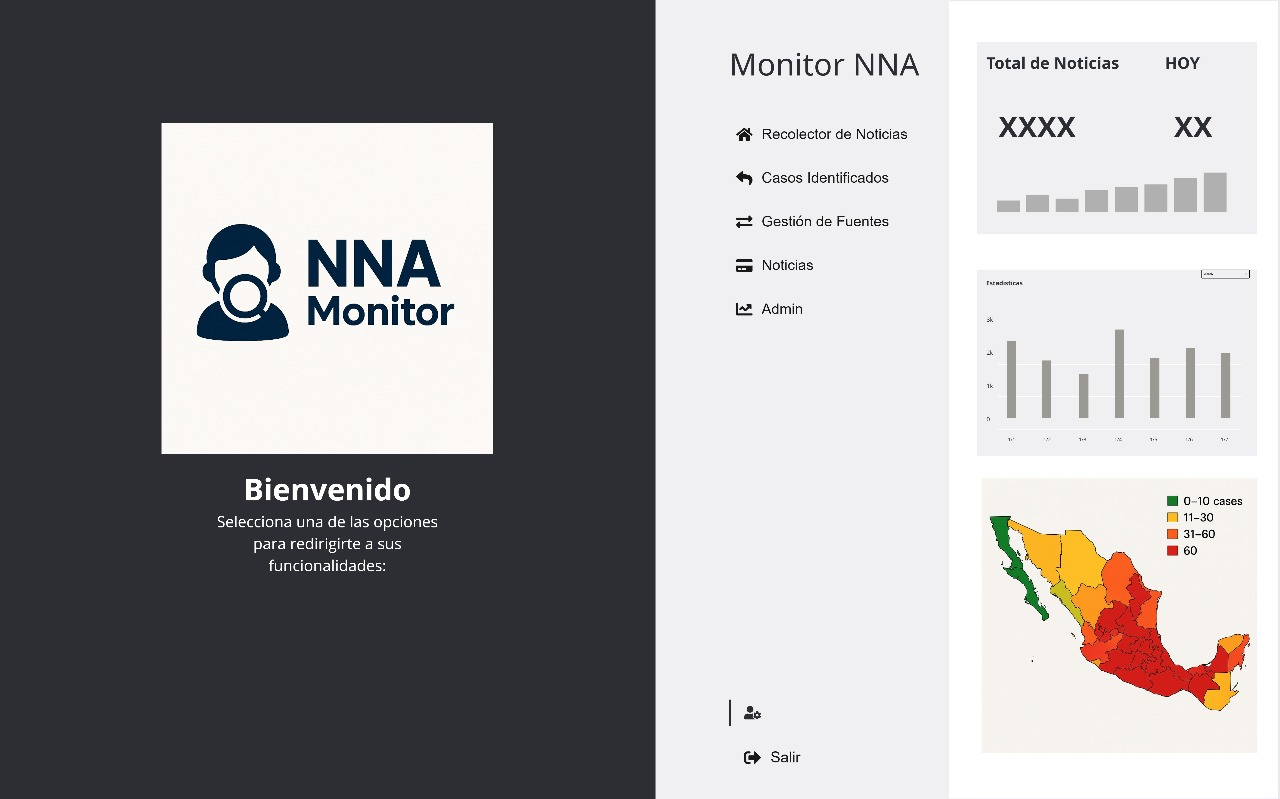
\includegraphics[width=0.7\textwidth,keepaspectratio]{media/Mockup_home.jpg}
\caption{Mockup de la pantalla principal (Home)}
\label{fig:mockup_home}
\end{figure}

\subsection{Mockup de Resumen General}
\label{anexo:mockup_resumen}

Diseño de la pantalla de resumen general con estadísticas y métricas del sistema.

\begin{figure}[h]
\centering
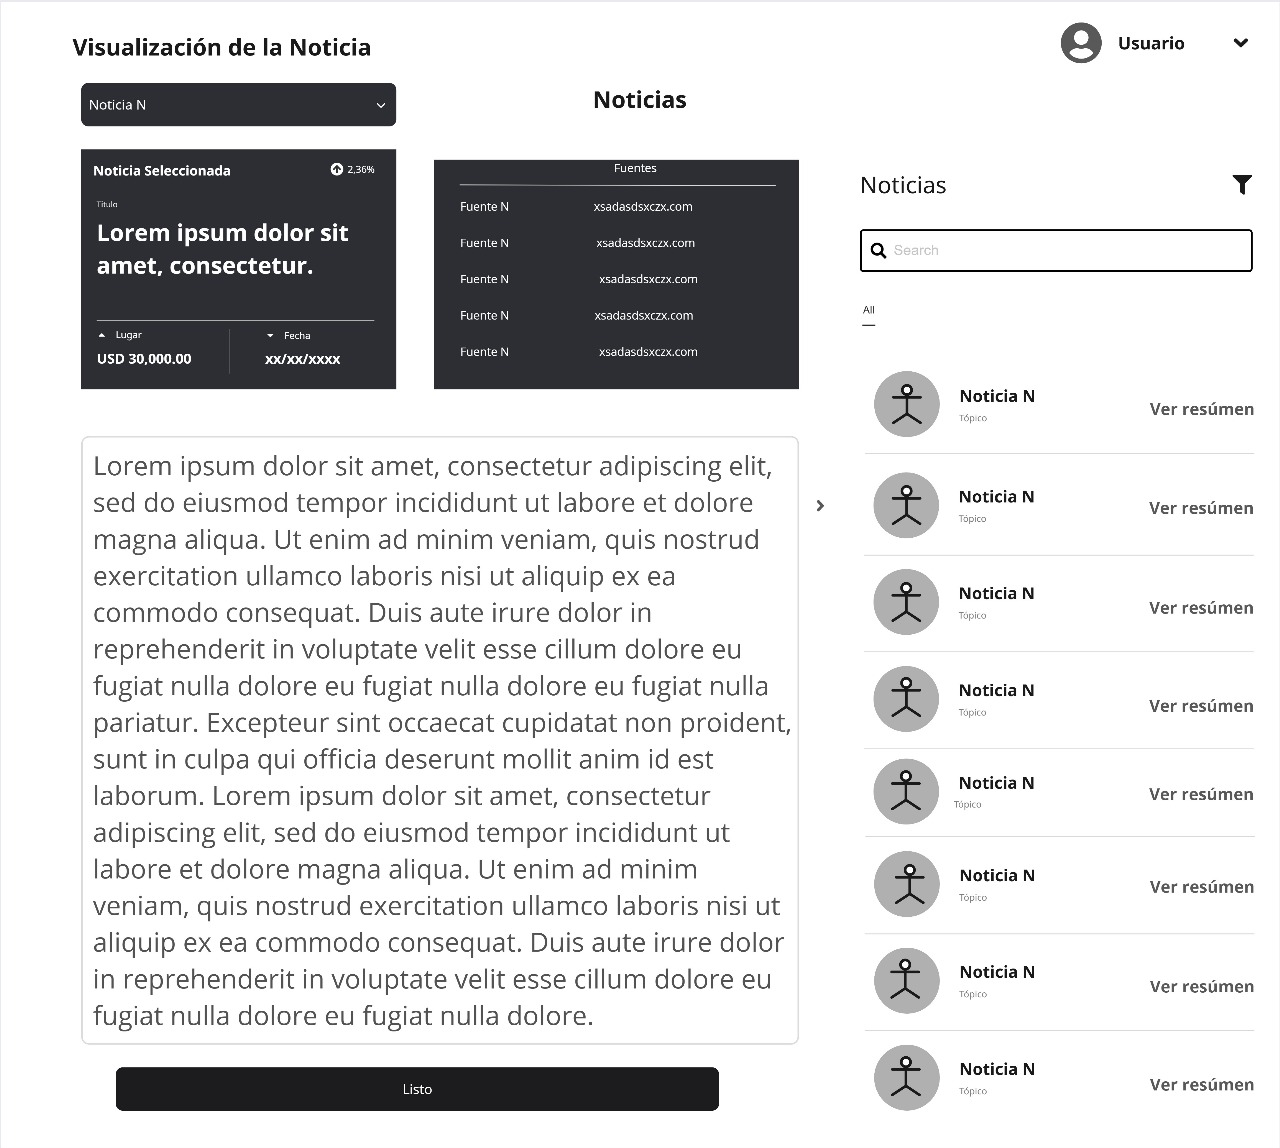
\includegraphics[width=0.7\textwidth,keepaspectratio]{media/Mockup_ResumenGeneral.jpg}
\caption{Mockup de la pantalla de resumen general}
\label{fig:mockup_resumen}
\end{figure}

\clearpage

\subsection{Mockup de Recolector de Noticias}
\label{anexo:mockup_recolector}

Diseño de la interfaz del módulo de recolección de noticias.

\begin{figure}[h]
\centering
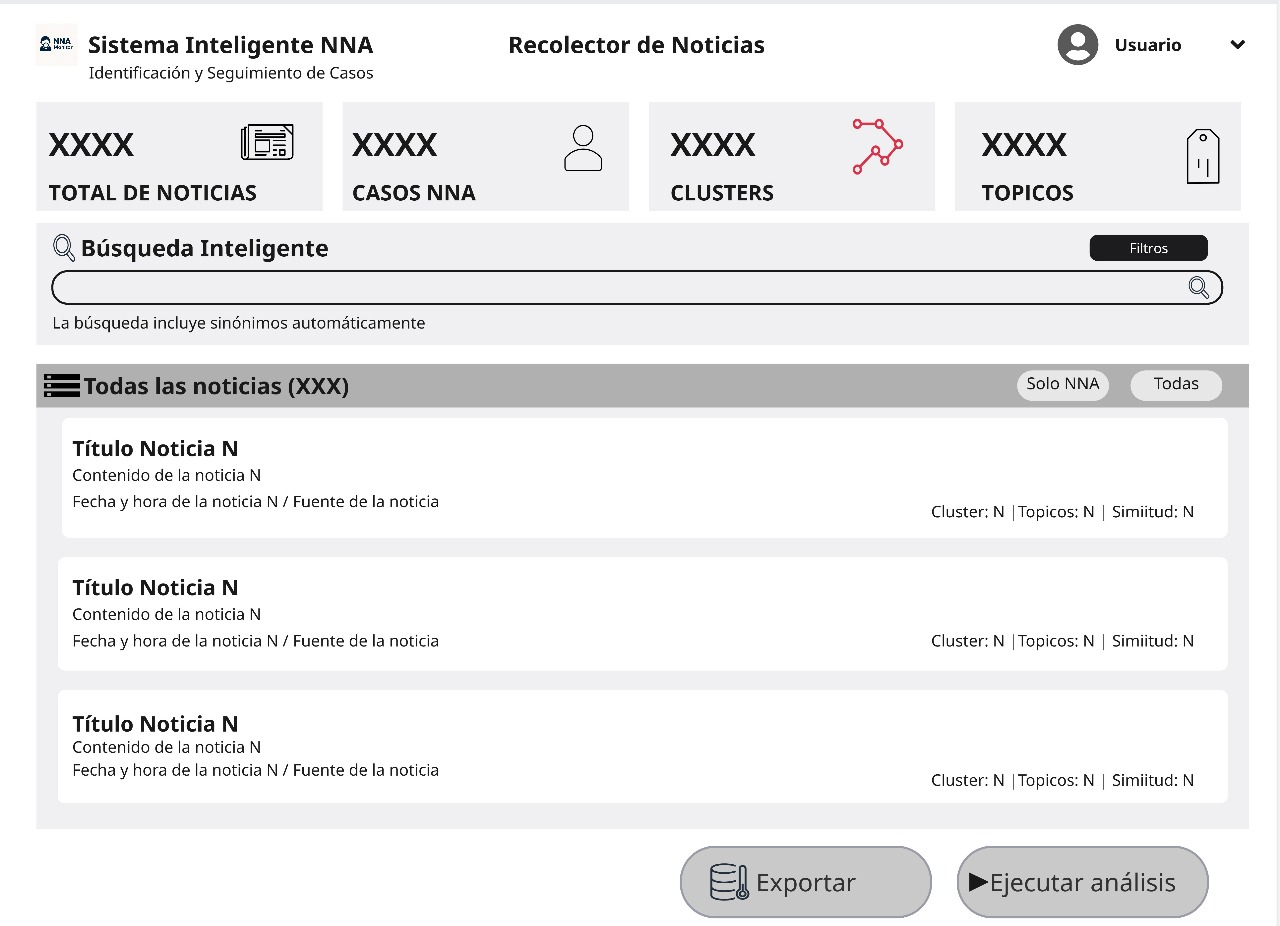
\includegraphics[width=0.7\textwidth,keepaspectratio]{media/Mockup_RecolectorNoticias.jpg}
\caption{Mockup del recolector de noticias}
\label{fig:mockup_recolector}
\end{figure}

\subsection{Mockup de Gestión de Fuentes}
\label{anexo:mockup_fuentes}

Diseño de la pantalla de gestión y configuración de fuentes de información.

\begin{figure}[h]
\centering
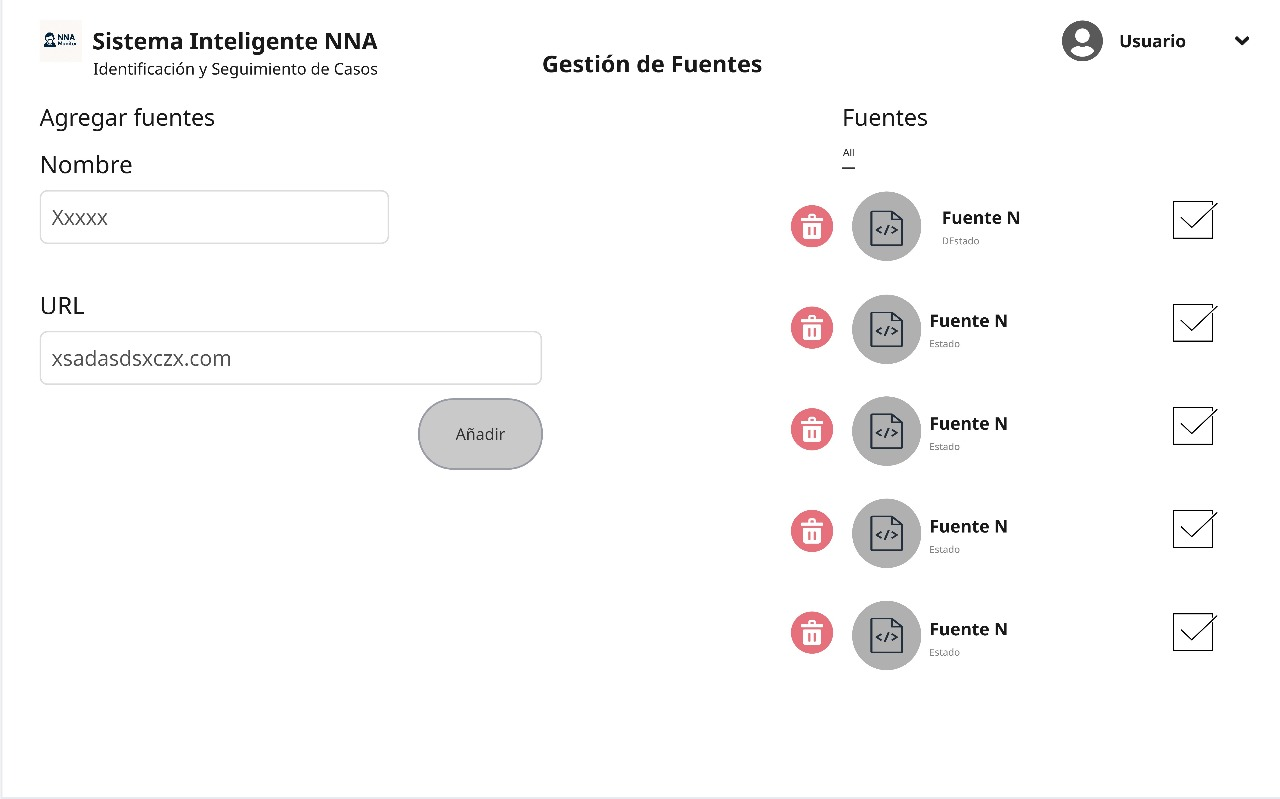
\includegraphics[width=0.7\textwidth,keepaspectratio]{media/Mockup_GestionFuentes.jpg}
\caption{Mockup de gestión de fuentes}
\label{fig:mockup_fuentes}
\end{figure}

\subsection{Mockup de Filtros}
\label{anexo:mockup_filtro}

Diseño de la interfaz de filtros para búsqueda y análisis de noticias.

\begin{figure}[h]
\centering
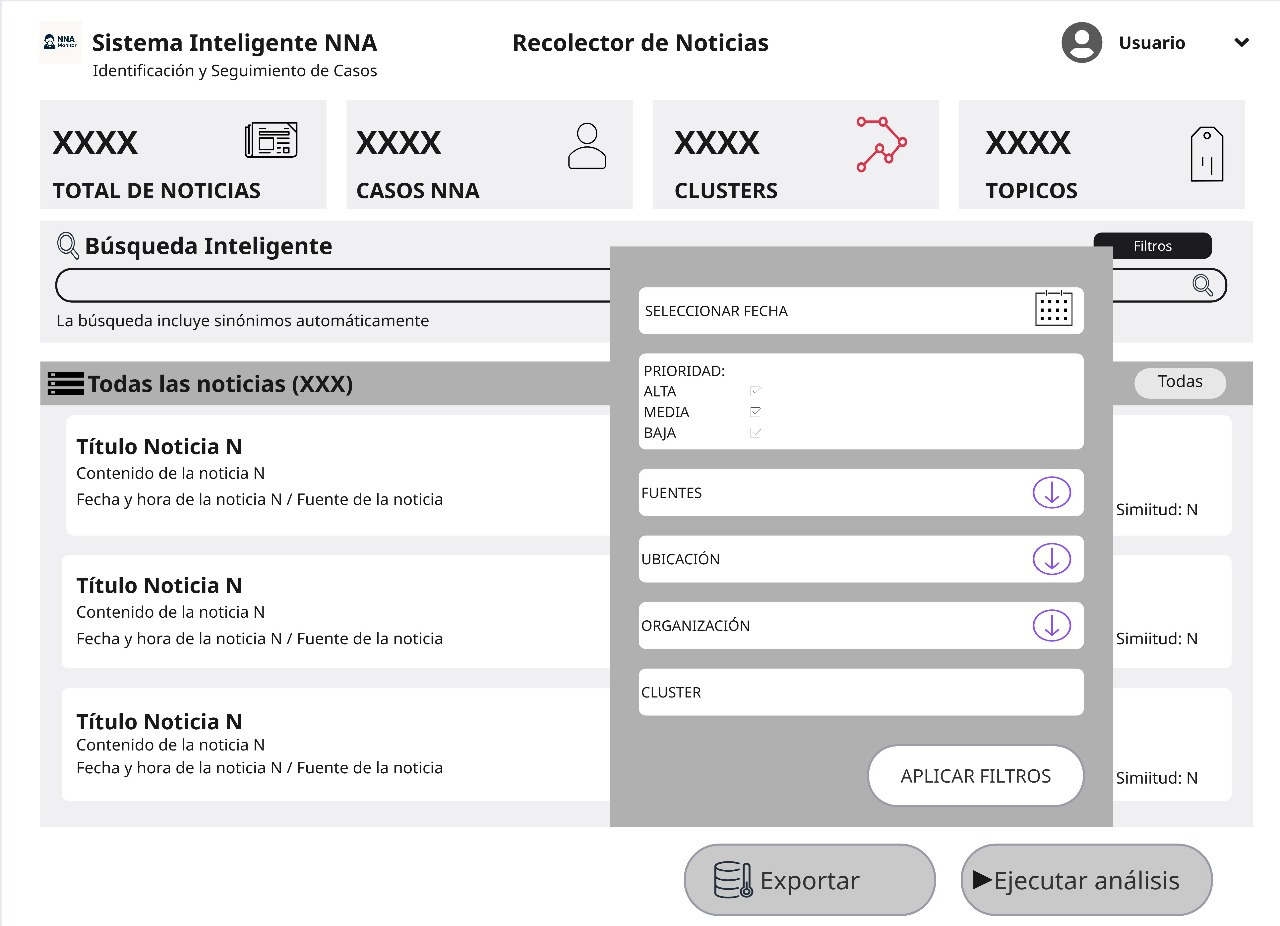
\includegraphics[width=0.7\textwidth,keepaspectratio]{media/Mockup_filtro.jpg}
\caption{Mockup de la pantalla de filtros}
\label{fig:mockup_filtro}
\end{figure}

\clearpage

\subsection{Mockup de Perfil de Usuario}
\label{anexo:mockup_perfil}

Diseño de la pantalla de perfil y configuración de usuario.

\begin{figure}[h]
\centering
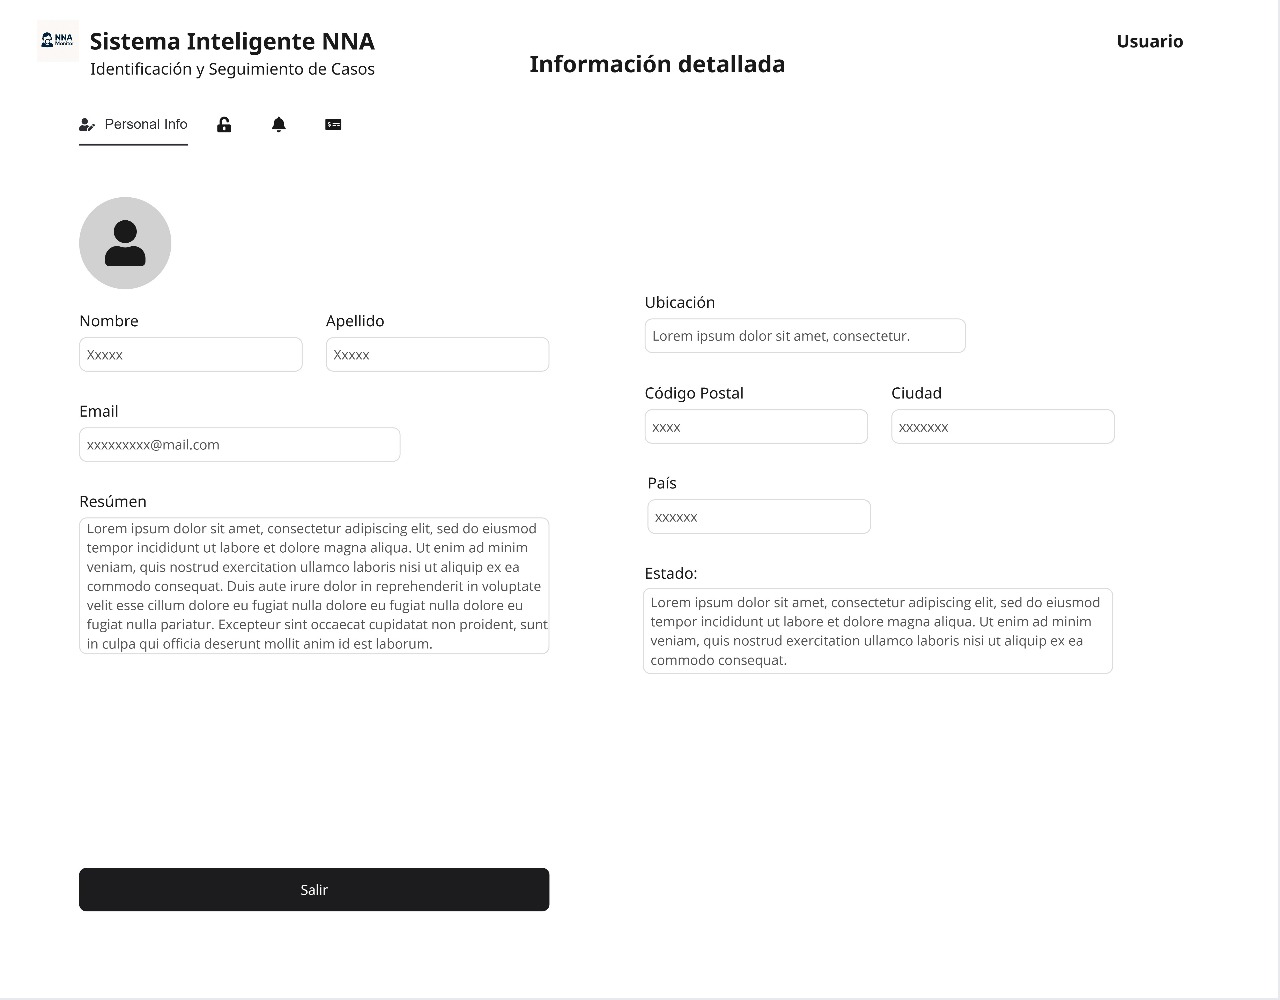
\includegraphics[width=0.7\textwidth,keepaspectratio]{media/Mockup_perfil.jpg}
\caption{Mockup del perfil de usuario}
\label{fig:mockup_perfil}
\end{figure}

\clearpage
